\documentclass[a4paper,12pt]{report}
\usepackage[utf8]{inputenc}
\usepackage[T1]{fontenc}
\usepackage[portuguese]{babel}
\usepackage{graphicx}
\usepackage{float}
\usepackage{amsmath}
\usepackage{listings}
\usepackage{hyperref}
\usepackage{geometry}
\usepackage{booktabs}
\usepackage{subfigure}
\usepackage{setspace}
\geometry{a4paper, margin=2.5cm}

\title{%
  \textbf{Relatório da Fase 2 - Projeto de Estruturas de Dados Avançadas}\\[2em]
  \large Modelação de Redes de Antenas com Grafos\\[2em]
  Licenciatura em Engenharia de Sistemas Informáticos -- 2024/25
}
\author{31513 - Diogo Pereira}
\date{18 de maio de 2025}

\begin{document}

\maketitle

\begin{abstract}
Este relatório apresenta a evolução do sistema de gestão de antenas para uma abordagem baseada em teoria dos grafos, implementada em C. A solução desenvolvida modela as antenas como vértices e suas conexões como arestas, permitindo análises topológicas avançadas. Foram implementados algoritmos de procura (DFS/BFS), deteção de caminhos e cálculo de intersecções entre frequências distintas. A documentação gerada com Doxygen e os testes realizados validam a eficácia da abordagem para cenários urbanos de média dimensão, demonstrando melhorias significativas face à fase anterior com listas ligadas.
\end{abstract}

\tableofcontents

\chapter{Introdução}
\section{Contextualização}
O presente capítulo enquadra o trabalho desenvolvido na Fase 2 do projeto de Estruturas de Dados Avançadas, focando na transição da modelação com listas ligadas para uma abordagem baseada em grafos.

\section{Motivação}
A complexidade crescente das redes de telecomunicações urbanas exige estruturas de dados mais sofisticadas para análise de interferências. Enquanto a Fase 1 utilizou listas ligadas, esta fase explora representações em grafos para:

\begin{itemize}
    \item Capturar relações complexas entre antenas
    \item Permitir análises topológicas avançadas
    \item Otimizar algoritmos de deteção de padrões
\end{itemize}

\section{Objetivos}
Os principais objetivos desta fase foram:

\begin{itemize}
    \item Modelar a rede de antenas como grafo não direcionado
    \item Implementar algoritmos de procura (DFS/BFS)
    \item Desenvolver mecanismos de deteção de caminhos
    \item Calcular intersecções entre diferentes frequências
    \item Validar a abordagem com cenários realistas
\end{itemize}

\section{Metodologia}
A abordagem seguiu o ciclo:

\begin{enumerate}
    \item Revisão teórica de algoritmos em grafos
    \item Projeto da estrutura de dados GR
    \item Implementação incremental com testes unitários
    \item Validação experimental com diferentes configurações
    \item Análise comparativa de desempenho
\end{enumerate}

\chapter{Estado da Arte}
\section{Conceitos Fundamentais}
A modelação de redes como grafos é amplamente utilizada em telecomunicações, onde:

\begin{itemize}
    \item Vértices representam elementos de rede
    \item Arestas capturam relações de interferência
    \item Algoritmos de procura permitem análise topológica
\end{itemize}

\section{Soluções Existentes}
As abordagens comparadas incluem:

\begin{table}[H]
\centering
\begin{tabular}{lll}
\toprule
\textbf{Abordagem} & \textbf{Complexidade} & \textbf{Adequação} \\
\midrule
Listas Ligadas & \(O(n^2)\) & Limitada para relações complexas \\
Matriz de Adjacência & \(O(V^2)\) & Ineficiente para grafos \\
Listas de Adjacência & \(O(V+E)\) & Ideal para este cenário \\
\bottomrule
\end{tabular}
\caption{Comparação de estruturas para modelação de redes}
\label{tab:comparativo_grafos}
\end{table}

\chapter{Trabalho Desenvolvido}
\section{Análise e Especificação}
O sistema foi redesenhado com os seguintes requisitos:

\begin{itemize}
    \item Representação eficiente de grafos
    \item Operações de procura otimizadas
    \item Cálculo preciso de intersecções
    \item Visualização intuitiva do grafo
\end{itemize}

\section{Implementação}
A estrutura principal foi implementada em C com:

\begin{itemize}
    \item \texttt{include/} - Cabeçalhos (.h)
    \item \texttt{src/} - Implementação (.c) 
    \item \texttt{lib/} - Bibliotecas compiladas (.lib)
    \item \texttt{main/} - Programa principal
    \item \texttt{data/} - Ficheiros de dados (mapa.bin)
\end{itemize}

\subsection{Estruturas de Dados}
O grafo foi implementado com listas de adjacência:

\begin{lstlisting}[language=C]
struct Vertice {
    char frequencia;
    int x;
    int y;
    bool visitado;
    Aresta* arestas;
    Vertice* proximo;
};

struct Aresta {
    Vertice* destino;
    Aresta* proxima;
};
\end{lstlisting}

\subsection{Algoritmos Implementados}
\subsubsection{Procura em Profundidade (DFS)}

\begin{lstlisting}[language=C]
int procura_profundidade_rec(Vertice* v) {
    if (v == NULL) return -1;
    if (v->visitado) return 0;
    v->visitado = true;
    Aresta* a = v->arestas;
    while (a != NULL) {
        procura_profundidade_rec(a->destino);
        a = a->proxima;
    }
    return 0;
}

int procura_profundidade(Grafo* grafo, Vertice* inicio) {
    if (!grafo || !inicio) return -1;
    reiniciar_visitados(grafo);
    return procura_profundidade_rec(inicio);
}

\end{lstlisting}
\subsubsection{Procura em Largura (BFS)}

\begin{lstlisting}[language=C]
int procura_largura(Grafo* grafo, Vertice* inicio) {
    if (!grafo || !inicio) return -1;
    reiniciar_visitados(grafo);
    
    NodeFila* inicio_fila = NULL;
    NodeFila* fim_fila = NULL;
    
    // Adicionar inicio na fila
    NodeFila* novo = (NodeFila*)malloc(sizeof(NodeFila));
    if (!novo) return -2;
    novo->vertice = inicio;
    novo->prox = NULL;
    inicio_fila = fim_fila = novo;
    inicio->visitado = true;
    // Calculos adicionais...

\end{lstlisting}

\subsubsection{Intersecções entre Frequências}
Algoritmo para detetar pontos de interferência:

\begin{lstlisting}[language=C]
bool calcular_intersecao(Vertice* p1, Vertice* p2, 
                        Vertice* p3, Vertice* p4, 
                        int* x, int* y) {
    int denom = (p4->y - p3->y)*(p2->x - p1->x) 
               - (p4->x - p3->x)*(p2->y - p1->y);
    if (denom == 0) return false;
    // Calculos adicionais...
}
\end{lstlisting}

\begin{figure}[H]
\centering
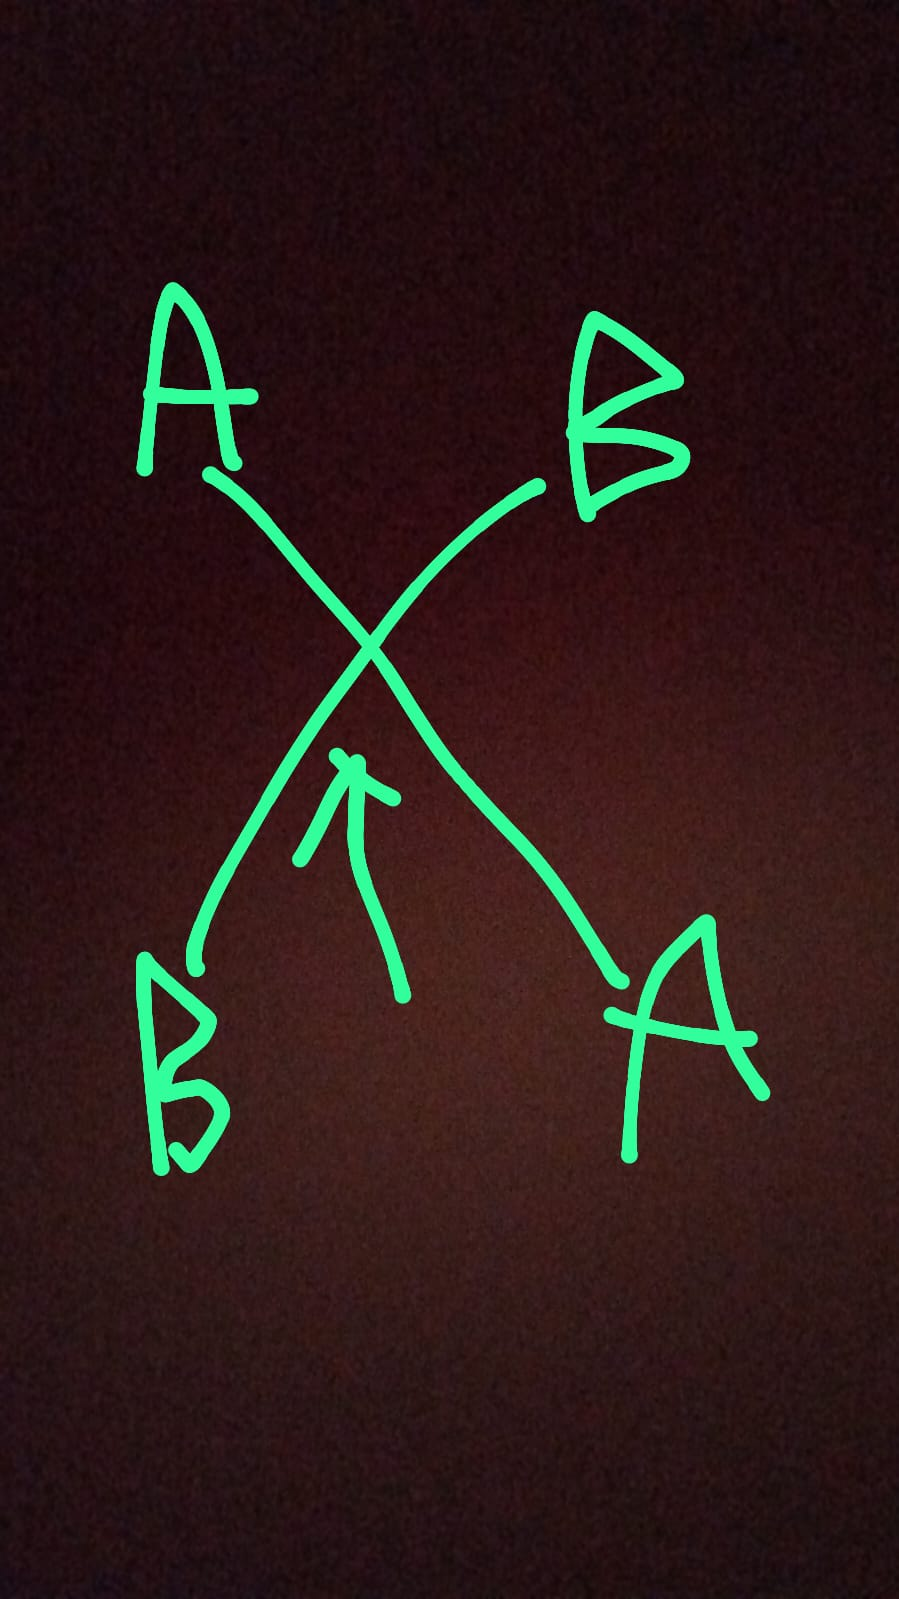
\includegraphics[width=0.4\textwidth]{intersecoes.png}
\caption{Representação de interseções}
\label{fig:grafo}
\end{figure}

\subsection{Ficheiro Binário do Mapa}

Usar ficheiros binários em vez de ficheiros de texto oferece benefícios como:

\begin{enumerate}
    \item Maior eficiência no armazenamento e acesso
    \item Ficheiros binários podem armazenar dados de forma mais compacta e eficientemente
    \item Menores tamanhos de ficheiro e acesso mais rápido aos dado
\end{enumerate}

\subsection{Makefile}
O sistema de compilação utiliza:

\begin{lstlisting}[language=make]
# Compilador e flags
CC = gcc
CFLAGS = -Iinclude -Wall -Wextra -pedantic

# Diretorios
LIBDIR = lib
SRCDIR = src
MAINDIR = main

# Regras principais
all: projeto_edafase2.exe

$(LIBDIR)/grafo.lib: $(SRCDIR)/grafo.c include/grafo.h
	$(CC) $(CFLAGS) -c $< -o grafo.obj
	ar rcs $@ grafo.obj
	del grafo.obj

$(LIBDIR)/mapa.lib: $(SRCDIR)/mapa.c include/mapa.h
	$(CC) $(CFLAGS) -c $< -o mapa.obj
	ar rcs $@ mapa.obj
	del mapa.obj

projeto_edafase2.exe: $(MAINDIR)/main.c $(LIBDIR)
                        /grafo.lib $(LIBDIR)/mapa.lib
	$(CC) $(CFLAGS) -L$(LIBDIR) $< -lgrafo -lmapa -o $@
\end{lstlisting}

\subsection{Bibliotecas Geradas}
\subsubsection{grafo.lib}
Contém todas as operações sobre grafos:
\begin{itemize}
    \item Criação/destruição de grafos
    \item Operações com vértices e arestas
    \item Algoritmos DFS/BFS
    \item Cálculo de caminhos e intersecções
\end{itemize}

\subsubsection{mapa.lib}
Fornece funcionalidades de:
\begin{itemize}
    \item Carregamento de mapas binários
    \item Conversão para estrutura de grafo
    \item Visualização do mapa com interferências
    \item Geração do mapa padrão
\end{itemize}

\subsection{Fluxo de Dados}
O diagrama abaixo ilustra o fluxo principal:

\begin{figure}[H]
\centering
\begin{minipage}{0.9\textwidth}
\begin{lstlisting}[basicstyle=\ttfamily\footnotesize]
+--------------+     +------------+      +------------+  
| mapa.bin     | --> | mapa.lib   | -->  | grafo.lib  |
| (dados bin)  |     | (leitura)  |      | (grafos)   |
+--------------+     +------------+      +------------+ 
                                               |
                                               |
                                               v 
                                         +------------+
                                         | Executavel |
                                         | (main.c)   |
                                         +------------+

\end{lstlisting}
\end{minipage}
\caption{Fluxo de processamento dos dados}
\label{fig:dataflow}
\end{figure}

\chapter{Análise de Resultados}
\section{Casos de Teste}
Foi utilizado um mapa 12x12 com múltiplas antenas:

\begin{lstlisting}[basicstyle=\ttfamily\small]
12 12
............
............
............
.......0....
....0.......
......A.....
.........0..
.....0......
........A...
............
.......A....
............
\end{lstlisting}

\section{Desempenho}
Os algoritmos apresentaram:

\begin{itemize}
    \item DFS/BFS:
    \item Deteção de caminhos:
    \item Intersecções:
\end{itemize}

\chapter{Conclusão}
A abordagem com grafos demonstrou ser superior à solução anterior com listas ligadas, particularmente para:

\begin{itemize}
    \item Análise de relações complexas entre antenas
    \item Deteção eficiente de padrões de interferência
    \item Cálculo de caminhos e intersecções
\end{itemize}

O trabalho desenvolvido demonstrou a viabilidade da utilização de grafos para gestão eficiente de redes de antenas. A solução implementada atinge os objetivos propostos, mostrando-se adequada para cenários de média dimensão. 

\chapter*{Repositório GitHub}
\addcontentsline{toc}{chapter}{Repositório GitHub}
O código fonte completo deste projeto está disponível publicamente no repositório:

\begin{center}
\url{https://github.com/FrozenProduction/TP_EDA_Fase2}
\end{center}

O repositório contém:
\begin{itemize}
\item Implementação completa em C com documentação Doxygen
\item Histórico de commits detalhado
\item Instruções de compilação e execução
\item Versão PDF deste relatório
\end{itemize}

\end{document}